\section{实验结果}
\label{sec:experiments}

我们进行了一系列实验,以验证来自 \cref{sec:theory} 的分析结果的泛化能力。  
所有实验均在本地的单核 CPU 机器或计算集群上运行。  
由于所有数据集均为程序生成,训练过程依赖于模型结构以及数据采样的复杂性,  
但每次模拟运行的训练时间在 10 到 60 分钟之间。
\subsection{通过正负预测验证 Claim~\labelcref{thm:localization}}
\label{sec:theory-validation}
\newcommand{\sampleheight}{42pt}
\newcommand{\covheight}{46pt}
\newcommand{\marginalheight}{50pt}
\setlength{\tabcolsep}{4pt}
\begin{figure}[t]
  \centering
  \hspace{-1.2em}
  \scalebox{0.9}{
  \begin{centering}
    \begin{tabular}{p{51pt}
      @{\hspace{10pt}}m{2pt}l
      @{\hspace{5pt}}l
      @{\hspace{10pt}}m{2pt}l
      @{\hspace{10pt}}m{2pt}l}
        \raisebox{18pt}{\small$\texttt{Ising}$} &
        \raisebox{34pt}{\rotatebox{90}{\tiny input value}} &
        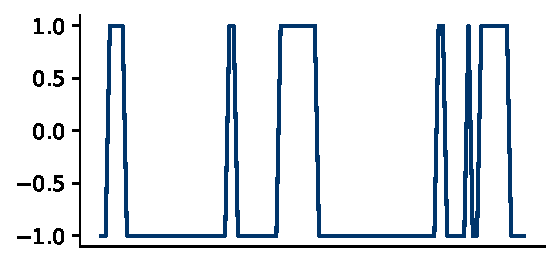
\includegraphics[height=\sampleheight]{figures/task/samples_long/ising.pdf} &
        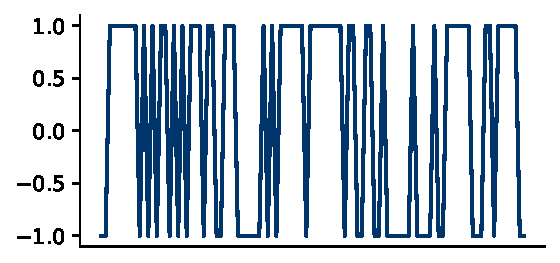
\includegraphics[height=\sampleheight]{figures/task/samples_short/ising.pdf} &
        \raisebox{38pt}{\rotatebox{90}{\tiny input dimension}} &
        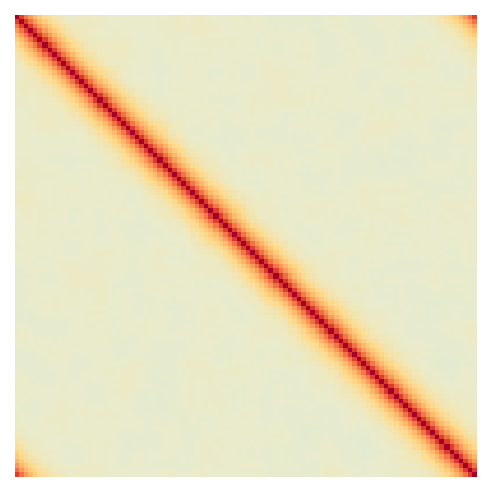
\includegraphics[height=\covheight]{figures/task/cov/ising.pdf} &
        \raisebox{40pt}{\rotatebox{90}{\tiny $p(X_i)$}} &
        \raisebox{-4pt}{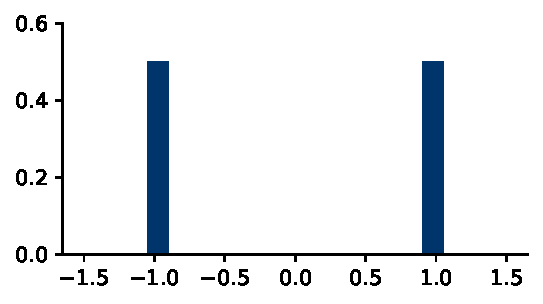
\includegraphics[height=\marginalheight]{figures/task/marginal/ising.pdf}} \\
        \noalign{\vskip -36pt}
        \raisebox{18pt}{\small$\texttt{NLGP}(0.01)$} &
        \raisebox{34pt}{\rotatebox{90}{\tiny input value}} &
        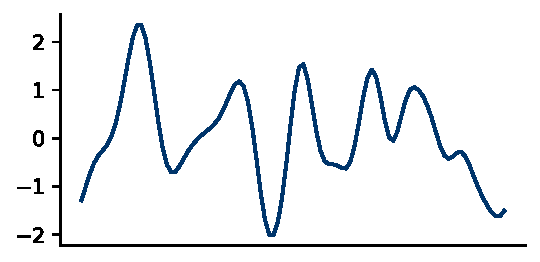
\includegraphics[height=\sampleheight]{figures/task/samples_long/gaussian.pdf} &
        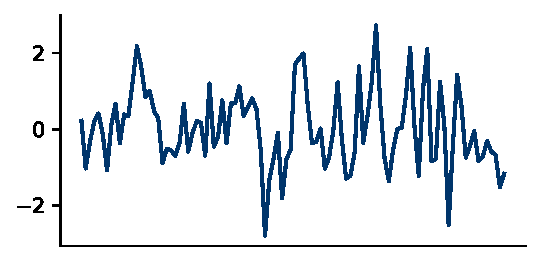
\includegraphics[height=\sampleheight]{figures/task/samples_short/gaussian.pdf} &
        \raisebox{38pt}{\rotatebox{90}{\tiny input dimension}} &
        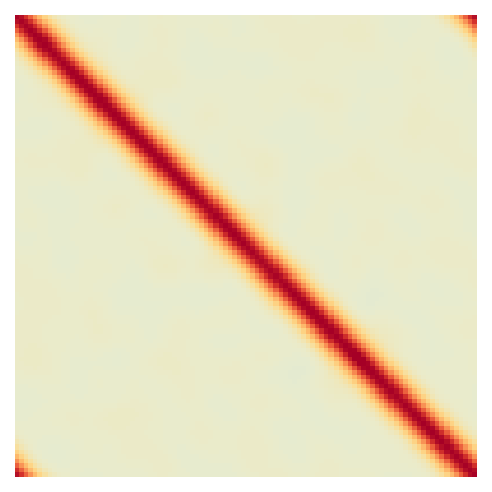
\includegraphics[height=\covheight]{figures/task/cov/gaussian.pdf} &
        \raisebox{40pt}{\rotatebox{90}{\tiny $p(X_i)$}} &
        \raisebox{-4pt}{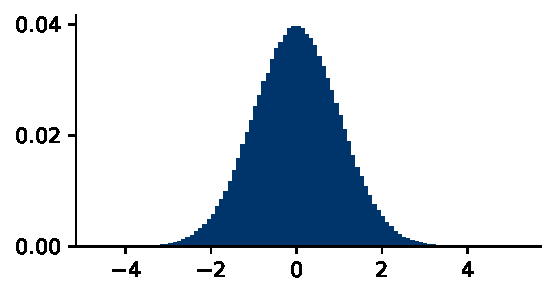
\includegraphics[height=\marginalheight]{figures/task/marginal/gaussian.pdf}} \\
        \noalign{\vskip -36pt}
        \raisebox{18pt}{\small $\texttt{Kur}(5)$} &
        \raisebox{34pt}{\rotatebox{90}{\tiny input value}} &
        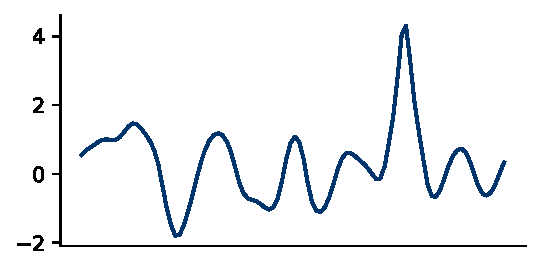
\includegraphics[height=\sampleheight]{figures/task/samples_long/alg5.pdf} &
        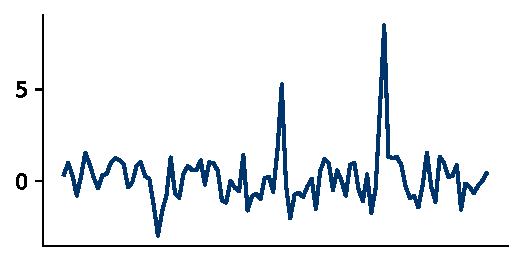
\includegraphics[height=\sampleheight]{figures/task/samples_short/alg5.pdf} &
        \raisebox{38pt}{\rotatebox{90}{\tiny input dimension}} &
        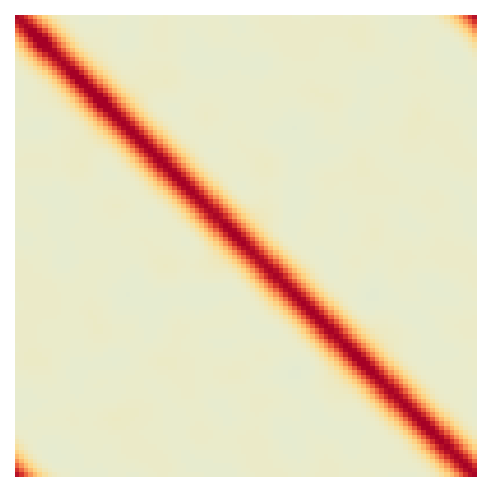
\includegraphics[height=\covheight]{figures/task/cov/alg5.pdf} &
        \raisebox{40pt}{\rotatebox{90}{\tiny $p(X_i)$}} &
        \raisebox{-4pt}{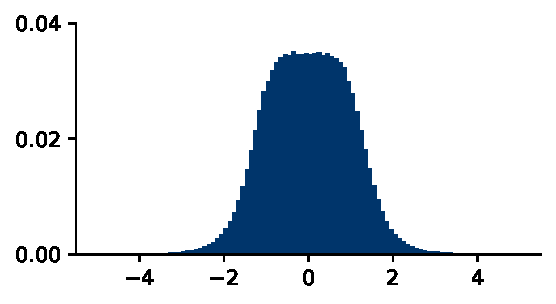
\includegraphics[height=\marginalheight]{figures/task/marginal/alg5.pdf}} \\
        \noalign{\vskip -37pt}
        &&
        \hspace{25pt}\tiny input dimension &
        \hspace{25pt}\tiny input dimension & &
        \hspace{3pt}\tiny input dimension & &
        \hspace{37pt}\tiny input value \\
  \end{tabular}
  \end{centering}
  }
  \caption{
    从左到右:
    长尺度和短尺度样本 $\mathbf{x}$,
    单一尺度的协方差 $\Sigma$,
    以及数据模型的边缘分布 $p(X_i)$,如 \cref{sec:task} 所述:
    Ising 模型(左、右样本分别为 $J=1.2, 0.3$),
    非线性高斯过程~\parencite[NLGP;~][]{ingrosso2022data},
    以及可控峰度模型 \texttt{Kur}
    (左、右样本分别为 $\xi=5, 1$)。
    \emph{
    每个模型生成的样本以零为中心,且其协方差可以被约束为相似,
    但具有不同的高阶统计量,从维度方向的边缘分布中可以看出这一点。
    }
}
  \label{fig:task}
  \vspace{-10pt}
\end{figure}


在 \cref{fig:replications} 中,我们首先通过单神经元模型(\labelcref{item:single-neuron-model})验证了 Claim~\labelcref{thm:localization},该模型在 $\texttt{NLGP}(g)$ 和 $\texttt{Kur}(k)$ 数据模型的一系列超额峰度条件下进行了 30 个初始条件的训练。
我们使用在 \cref{app:IPR} 中定义的反参与比(IPR)。
这一度量也被 \textcite{ingrosso2022data} 使用,当仅有少量权重维度“参与”(具有较大幅值)时,其值较大;当权重维度的幅值分布较为均匀时,其值较小。
我们观察到,当 $g$ 和 $k$ 的取值导致负的超额峰度时,IPR 接近其最大值 $1.0$,表明权重是局域化的;而当超额峰度为正时,IPR 几乎为零,表明权重\emph{不}是局域化的。
IPR 在不同随机初始化下表现出极高的一致性,表明局域化由数据统计特性决定,而非初始化。
在 IPR 与超额峰度之间的趋势在 $\texttt{NLGP}(g)$ 和 $\texttt{Kur}(k)$ 数据模型中非常相似,这表明超额峰度是驱动局域化的主要因素,且局域化在很大程度上独立于数据分布的其他属性。
\newcommand{\sampleheight}{42pt}
\newcommand{\covheight}{46pt}
\newcommand{\marginalheight}{50pt}
\setlength{\tabcolsep}{4pt}
\begin{figure}[t]
  \centering
  \hspace{-1.2em}
  \scalebox{0.9}{
  \begin{centering}
    \begin{tabular}{p{51pt}
      @{\hspace{10pt}}m{2pt}l
      @{\hspace{5pt}}l
      @{\hspace{10pt}}m{2pt}l
      @{\hspace{10pt}}m{2pt}l}
        \raisebox{18pt}{\small$\texttt{Ising}$} &
        \raisebox{34pt}{\rotatebox{90}{\tiny input value}} &
        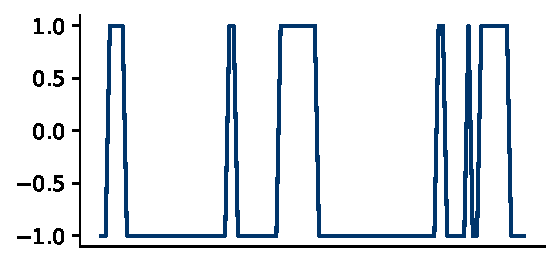
\includegraphics[height=\sampleheight]{figures/task/samples_long/ising.pdf} &
        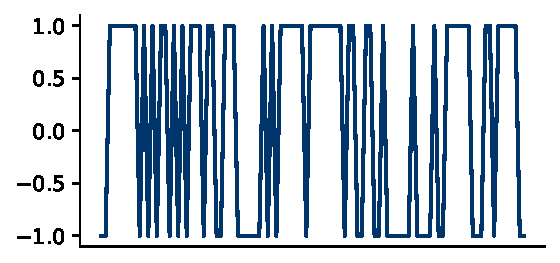
\includegraphics[height=\sampleheight]{figures/task/samples_short/ising.pdf} &
        \raisebox{38pt}{\rotatebox{90}{\tiny input dimension}} &
        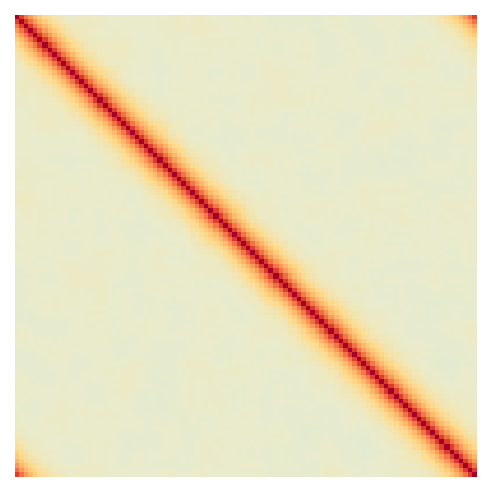
\includegraphics[height=\covheight]{figures/task/cov/ising.pdf} &
        \raisebox{40pt}{\rotatebox{90}{\tiny $p(X_i)$}} &
        \raisebox{-4pt}{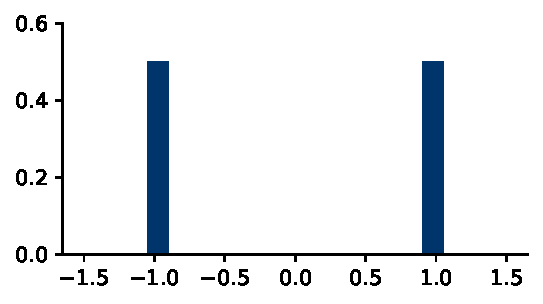
\includegraphics[height=\marginalheight]{figures/task/marginal/ising.pdf}} \\
        \noalign{\vskip -36pt}
        \raisebox{18pt}{\small$\texttt{NLGP}(0.01)$} &
        \raisebox{34pt}{\rotatebox{90}{\tiny input value}} &
        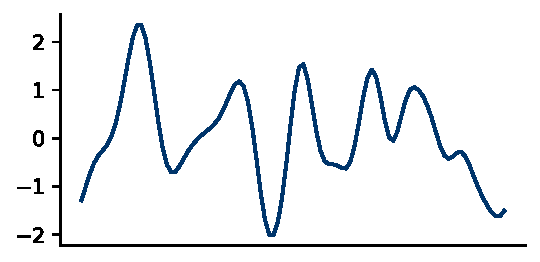
\includegraphics[height=\sampleheight]{figures/task/samples_long/gaussian.pdf} &
        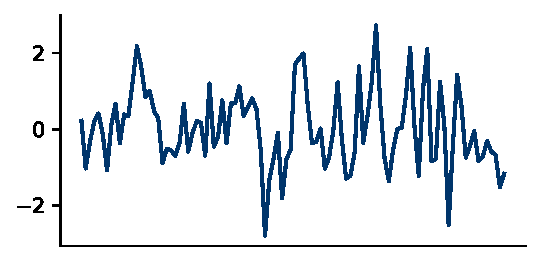
\includegraphics[height=\sampleheight]{figures/task/samples_short/gaussian.pdf} &
        \raisebox{38pt}{\rotatebox{90}{\tiny input dimension}} &
        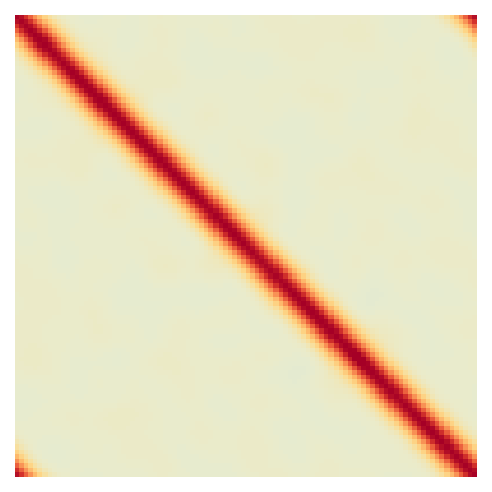
\includegraphics[height=\covheight]{figures/task/cov/gaussian.pdf} &
        \raisebox{40pt}{\rotatebox{90}{\tiny $p(X_i)$}} &
        \raisebox{-4pt}{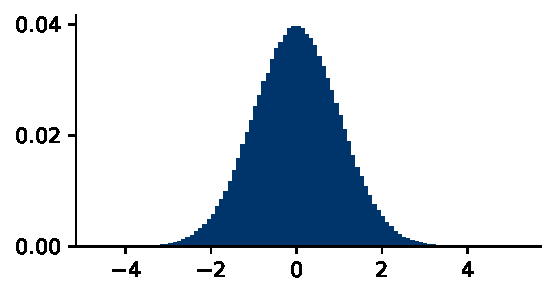
\includegraphics[height=\marginalheight]{figures/task/marginal/gaussian.pdf}} \\
        \noalign{\vskip -36pt}
        \raisebox{18pt}{\small $\texttt{Kur}(5)$} &
        \raisebox{34pt}{\rotatebox{90}{\tiny input value}} &
        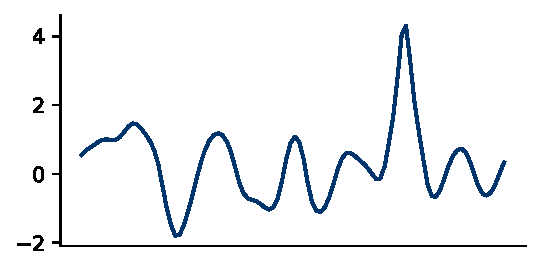
\includegraphics[height=\sampleheight]{figures/task/samples_long/alg5.pdf} &
        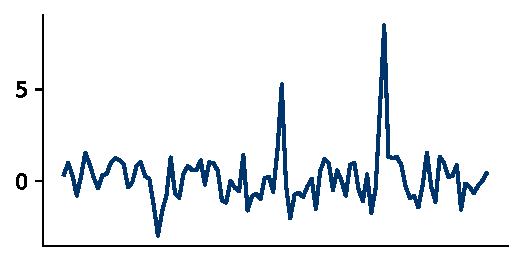
\includegraphics[height=\sampleheight]{figures/task/samples_short/alg5.pdf} &
        \raisebox{38pt}{\rotatebox{90}{\tiny input dimension}} &
        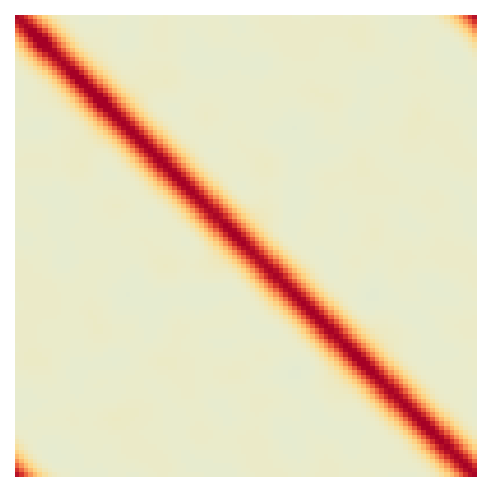
\includegraphics[height=\covheight]{figures/task/cov/alg5.pdf} &
        \raisebox{40pt}{\rotatebox{90}{\tiny $p(X_i)$}} &
        \raisebox{-4pt}{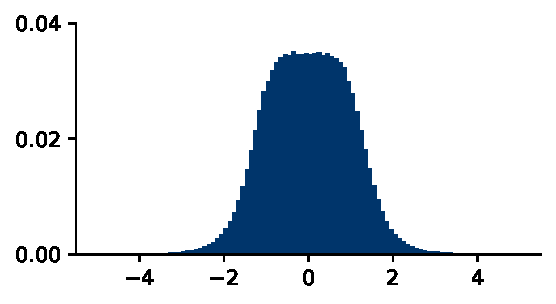
\includegraphics[height=\marginalheight]{figures/task/marginal/alg5.pdf}} \\
        \noalign{\vskip -37pt}
        &&
        \hspace{25pt}\tiny input dimension &
        \hspace{25pt}\tiny input dimension & &
        \hspace{3pt}\tiny input dimension & &
        \hspace{37pt}\tiny input value \\
  \end{tabular}
  \end{centering}
  }
  \caption{
    从左到右:
    长尺度和短尺度样本 $\mathbf{x}$,
    单一尺度的协方差 $\Sigma$,
    以及数据模型的边缘分布 $p(X_i)$,如 \cref{sec:task} 所述:
    Ising 模型(左、右样本分别为 $J=1.2, 0.3$),
    非线性高斯过程~\parencite[NLGP;~][]{ingrosso2022data},
    以及可控峰度模型 \texttt{Kur}
    (左、右样本分别为 $\xi=5, 1$)。
    \emph{
    每个模型生成的样本以零为中心,且其协方差可以被约束为相似,
    但具有不同的高阶统计量,从维度方向的边缘分布中可以看出这一点。
    }
}
  \label{fig:task}
  \vspace{-10pt}
\end{figure}


\Cref{fig:theory} 进一步通过具体示例验证了 Claim~\labelcref{thm:localization}。
我们在模型中保持相同的初始条件,并在 \texttt{Ising}、$\texttt{NLGP}(g=0.01)$ 和 $\texttt{Kur}(k=5)$ 数据模型上进行训练。
\texttt{Ising} 模型的边缘分布具有 $-2$ 的超额峰度,这是任何分布可能具有的最小值。
因此,我们观察到 \texttt{Ising}(左上)的放大器 $\varphi$ 是超线性的(深色实线在较大的 $a$ 上超过浅色虚线),这通过其在 \cref{eq:gradient_flow_early} 中的作用驱动了局域化。
将 \cref{eq:gradient_flow_early} 中的 $\varphi$ 通过三阶泰勒展开(红线)积分,得到的局域感受野与模拟结果(右侧两个面板)相似,验证了该近似的有效性。

对于其余导致振荡(正弦)型权重的分布(中间和底部行),由于其超额峰度为正,因此 Claim~\labelcref{thm:localization} 得到了验证。
动态稳态(最右侧)的取值比模拟结果(其左侧)更为负,
这一差异源于我们在 \cref{eq:gradient_flow_early} 中\emph{早期}梯度流的偏离,
但这些偏离仍足够温和,因此仍能恢复学习出的感受野的定性结构。

\newcommand{\sampleheight}{42pt}
\newcommand{\covheight}{46pt}
\newcommand{\marginalheight}{50pt}
\setlength{\tabcolsep}{4pt}
\begin{figure}[t]
  \centering
  \hspace{-1.2em}
  \scalebox{0.9}{
  \begin{centering}
    \begin{tabular}{p{51pt}
      @{\hspace{10pt}}m{2pt}l
      @{\hspace{5pt}}l
      @{\hspace{10pt}}m{2pt}l
      @{\hspace{10pt}}m{2pt}l}
        \raisebox{18pt}{\small$\texttt{Ising}$} &
        \raisebox{34pt}{\rotatebox{90}{\tiny input value}} &
        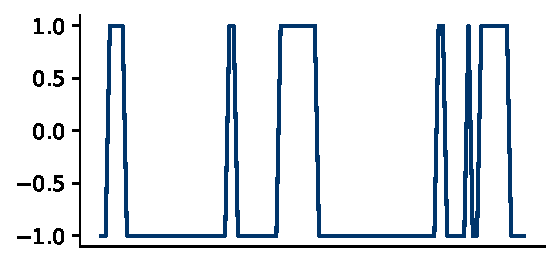
\includegraphics[height=\sampleheight]{figures/task/samples_long/ising.pdf} &
        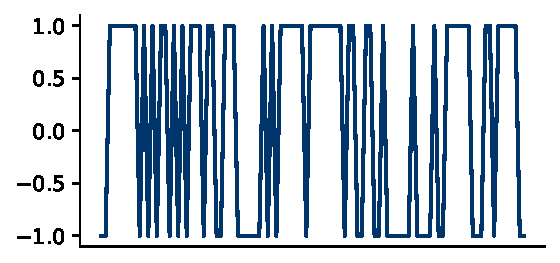
\includegraphics[height=\sampleheight]{figures/task/samples_short/ising.pdf} &
        \raisebox{38pt}{\rotatebox{90}{\tiny input dimension}} &
        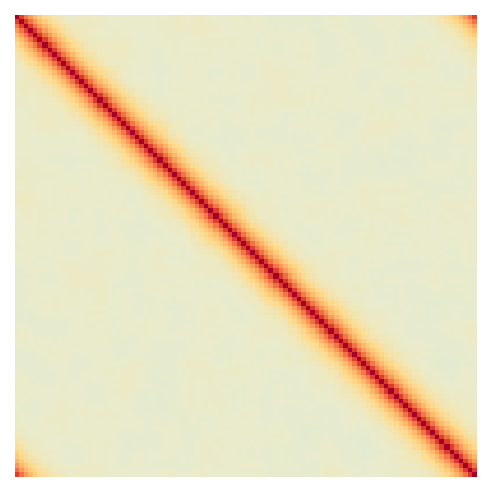
\includegraphics[height=\covheight]{figures/task/cov/ising.pdf} &
        \raisebox{40pt}{\rotatebox{90}{\tiny $p(X_i)$}} &
        \raisebox{-4pt}{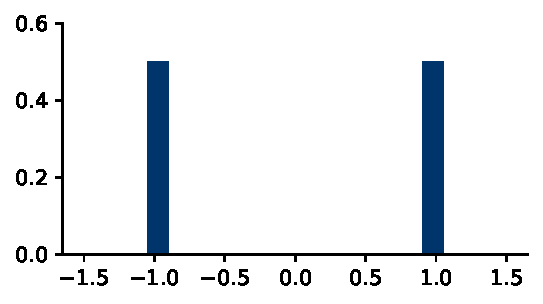
\includegraphics[height=\marginalheight]{figures/task/marginal/ising.pdf}} \\
        \noalign{\vskip -36pt}
        \raisebox{18pt}{\small$\texttt{NLGP}(0.01)$} &
        \raisebox{34pt}{\rotatebox{90}{\tiny input value}} &
        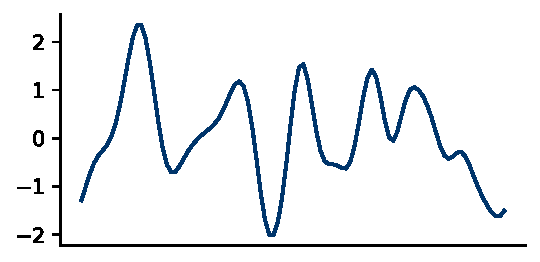
\includegraphics[height=\sampleheight]{figures/task/samples_long/gaussian.pdf} &
        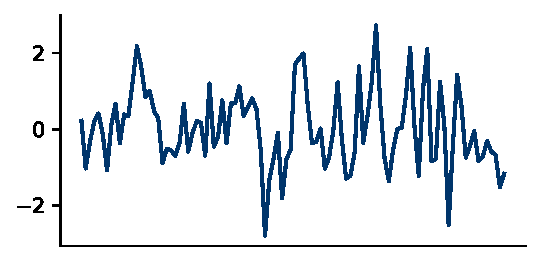
\includegraphics[height=\sampleheight]{figures/task/samples_short/gaussian.pdf} &
        \raisebox{38pt}{\rotatebox{90}{\tiny input dimension}} &
        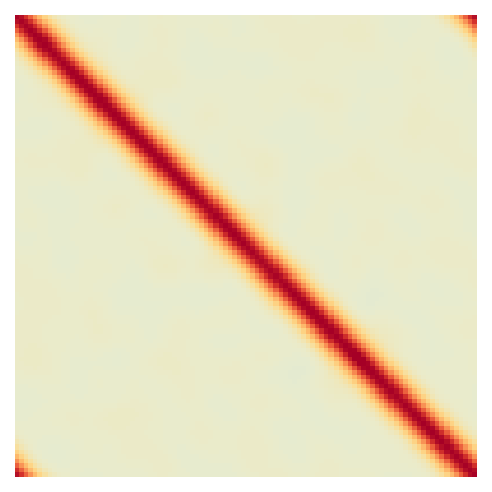
\includegraphics[height=\covheight]{figures/task/cov/gaussian.pdf} &
        \raisebox{40pt}{\rotatebox{90}{\tiny $p(X_i)$}} &
        \raisebox{-4pt}{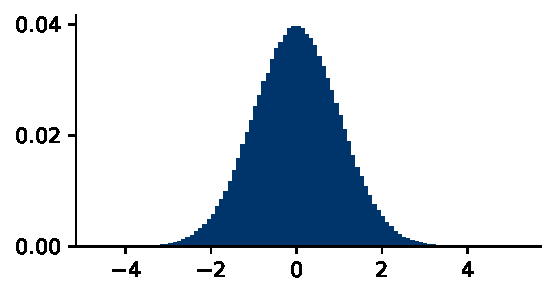
\includegraphics[height=\marginalheight]{figures/task/marginal/gaussian.pdf}} \\
        \noalign{\vskip -36pt}
        \raisebox{18pt}{\small $\texttt{Kur}(5)$} &
        \raisebox{34pt}{\rotatebox{90}{\tiny input value}} &
        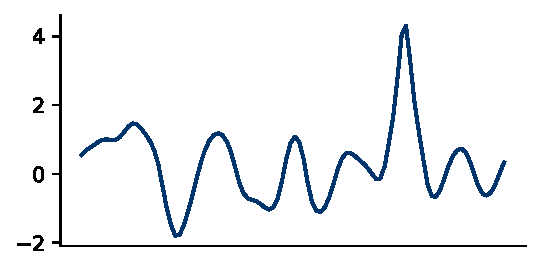
\includegraphics[height=\sampleheight]{figures/task/samples_long/alg5.pdf} &
        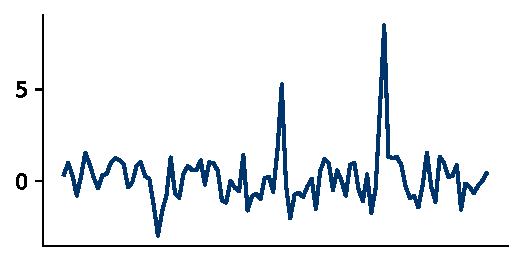
\includegraphics[height=\sampleheight]{figures/task/samples_short/alg5.pdf} &
        \raisebox{38pt}{\rotatebox{90}{\tiny input dimension}} &
        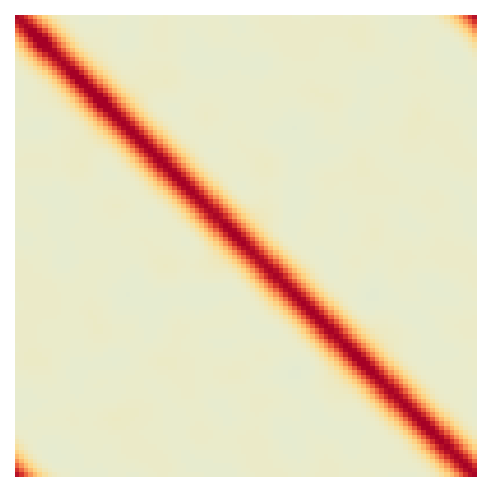
\includegraphics[height=\covheight]{figures/task/cov/alg5.pdf} &
        \raisebox{40pt}{\rotatebox{90}{\tiny $p(X_i)$}} &
        \raisebox{-4pt}{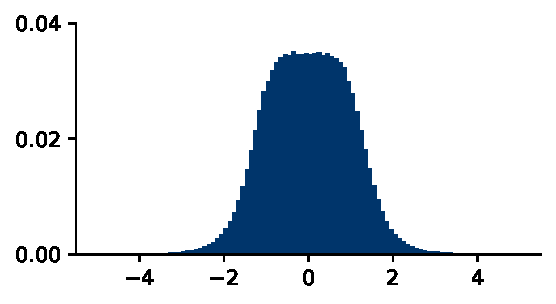
\includegraphics[height=\marginalheight]{figures/task/marginal/alg5.pdf}} \\
        \noalign{\vskip -37pt}
        &&
        \hspace{25pt}\tiny input dimension &
        \hspace{25pt}\tiny input dimension & &
        \hspace{3pt}\tiny input dimension & &
        \hspace{37pt}\tiny input value \\
  \end{tabular}
  \end{centering}
  }
  \caption{
    从左到右:
    长尺度和短尺度样本 $\mathbf{x}$,
    单一尺度的协方差 $\Sigma$,
    以及数据模型的边缘分布 $p(X_i)$,如 \cref{sec:task} 所述:
    Ising 模型(左、右样本分别为 $J=1.2, 0.3$),
    非线性高斯过程~\parencite[NLGP;~][]{ingrosso2022data},
    以及可控峰度模型 \texttt{Kur}
    (左、右样本分别为 $\xi=5, 1$)。
    \emph{
    每个模型生成的样本以零为中心,且其协方差可以被约束为相似,
    但具有不同的高阶统计量,从维度方向的边缘分布中可以看出这一点。
    }
}
  \label{fig:task}
  \vspace{-10pt}
\end{figure}

\subsection{通过位置预测验证\cref{eq:gradient_flow_early}}
\label{sec:peak-prediction}
在\cref{fig:theory}中的模拟和积分感受野表明,我们的分析模型能够有意义地再现神经网络训练中的感受野定位。
对于伊辛模型,我们看到积分甚至在与模拟相同的位置(在索引 $i=6$ 处)具有峰值,表明我们的近似具有精确性。
事实上,我们在28种不同的初始条件(权重初始化)下模拟了\cref{fig:theory}中的伊辛模型,并发现其中26种(93\%)的积分和模拟感受野的峰值完全匹配。
在两个峰值不同的情况下,它们的差异显著(参见\cref{fig:time}中的示例)。
\subsection{验证命题 \ref{thm:elliptical}:椭圆分布无法实现局部化}
\label{sec:elliptical-experiments}
命题 \ref{thm:elliptical} 指出,单神经元模型(\labelcref{item:single-neuron-model})在椭圆分布数据上训练时,将产生正弦形式的感受野,前提是 $\Sigma_0$ 和 $\Sigma_1$ 的谱满足一定条件。我们在 \cref{fig:elliptical} 中通过三种不同的椭圆分布验证了该结论。

第一种分布 $t_{40}(\nu=3)$ 所产生的预激活 $\langle \mathbf{w}, \mathbf{X} \rangle$ 具有 \emph{无限} 峰度,尽管如此,我们的理论仍预测最终的感受野将为正弦形式。该结论在 \cref{fig:elliptical} 中得到了验证,学习得到的感受野的确是一个周期为 1、截距为 0 的正弦函数。

我们还考虑了另一种从椭圆曲面上采样的数据,其方式是在 \cref{def:elliptical} 中固定 $R_y \equiv 1$。在这种情况下,我们观察到学习得到的感受野近似为常数函数 $-0.04$(注意 $\cos(2\pi \cdot 0 \cdot x) \equiv 1$ 是一个正弦函数,允许非零截距和常数函数)。

最后,我们考虑一种非常规的椭圆分布,其半径 $R$ 的密度为 $p_R(r) = (4e^{2r+4}) / (e^{2r}+e^{4})^{2} \cdot \mathbbm{1}(r \geq 2)$。该密度函数在 $r = 2$ 附近具有大部分概率质量,随后迅速衰减,从而对 $\mathbf{X}$ 施加了一个最小范数限制,并使其支持集中于椭圆曲面附近。如 \cref{fig:elliptical}(右)所示,该分布同样会产生震荡的稳态。

我们通过对最终的感受野拟合正弦函数验证了视觉观察,发现相对误差非常小。
\subsection{对多神经元模型和 ICA 的扩展}
\label{sec:extensions}

到目前为止,我们的所有分析都集中在使用 ReLU 激活函数的单神经元模型,并且未考虑从隐藏层到输出层的连接或偏置项,这些假设是为了使我们的分析更易处理而做出的。
在此,我们跳出这一假设范式,考虑 SCM 以及完整的两层网络(模型~\labelcref{item:many-neuron-model})。
在 \cref{fig:extensions}(左)和(中)中,我们在 $\texttt{Kur}(10)$ 和 $\texttt{Kur}(4)$ 数据集上训练了一个具有 10 个隐藏单元和 sigmoid 激活函数的 SCM,这两个数据集的超峭度分别为 $-0.93$ 和 $3.28$。
因此,根据我们对单神经元的分析,对于这些分布,我们分别\emph{预期会}和\emph{不会}观察到局部化现象。
这正是我们在 \cref{fig:extensions} 中观察到的结果:对于前者分布,其感受野呈现出明显的局部化特征;而对于后者分布,其感受野则表现为低频振荡。

\newcommand{\sampleheight}{42pt}
\newcommand{\covheight}{46pt}
\newcommand{\marginalheight}{50pt}
\setlength{\tabcolsep}{4pt}
\begin{figure}[t]
  \centering
  \hspace{-1.2em}
  \scalebox{0.9}{
  \begin{centering}
    \begin{tabular}{p{51pt}
      @{\hspace{10pt}}m{2pt}l
      @{\hspace{5pt}}l
      @{\hspace{10pt}}m{2pt}l
      @{\hspace{10pt}}m{2pt}l}
        \raisebox{18pt}{\small$\texttt{Ising}$} &
        \raisebox{34pt}{\rotatebox{90}{\tiny input value}} &
        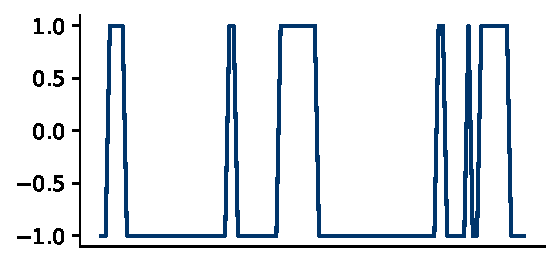
\includegraphics[height=\sampleheight]{figures/task/samples_long/ising.pdf} &
        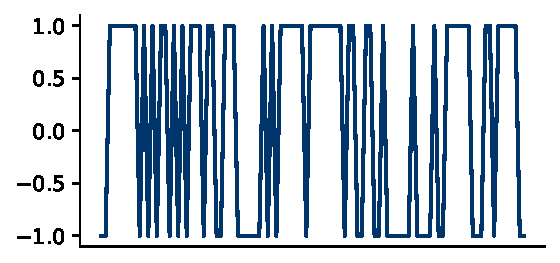
\includegraphics[height=\sampleheight]{figures/task/samples_short/ising.pdf} &
        \raisebox{38pt}{\rotatebox{90}{\tiny input dimension}} &
        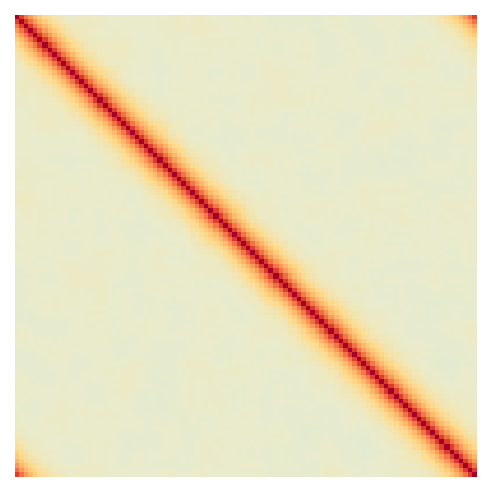
\includegraphics[height=\covheight]{figures/task/cov/ising.pdf} &
        \raisebox{40pt}{\rotatebox{90}{\tiny $p(X_i)$}} &
        \raisebox{-4pt}{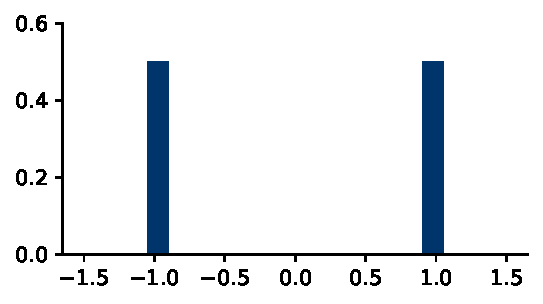
\includegraphics[height=\marginalheight]{figures/task/marginal/ising.pdf}} \\
        \noalign{\vskip -36pt}
        \raisebox{18pt}{\small$\texttt{NLGP}(0.01)$} &
        \raisebox{34pt}{\rotatebox{90}{\tiny input value}} &
        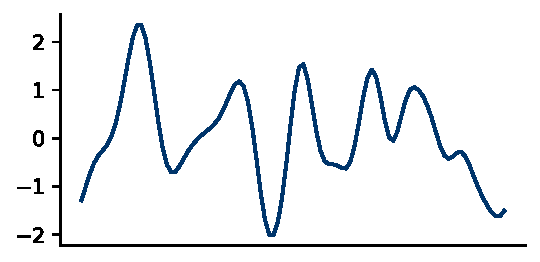
\includegraphics[height=\sampleheight]{figures/task/samples_long/gaussian.pdf} &
        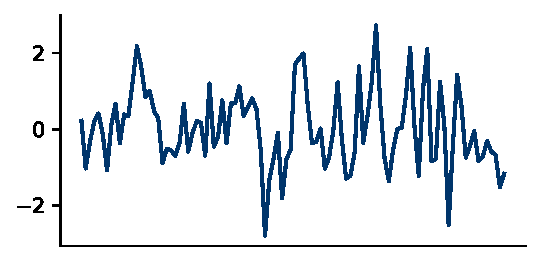
\includegraphics[height=\sampleheight]{figures/task/samples_short/gaussian.pdf} &
        \raisebox{38pt}{\rotatebox{90}{\tiny input dimension}} &
        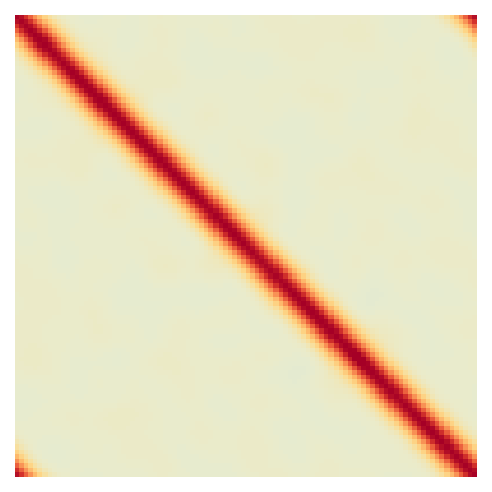
\includegraphics[height=\covheight]{figures/task/cov/gaussian.pdf} &
        \raisebox{40pt}{\rotatebox{90}{\tiny $p(X_i)$}} &
        \raisebox{-4pt}{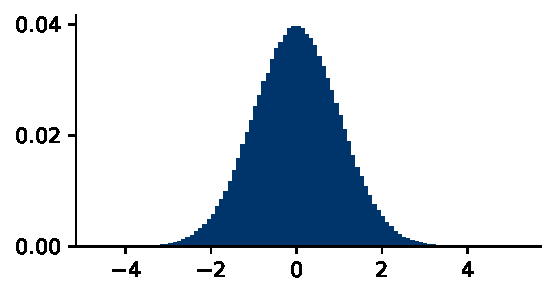
\includegraphics[height=\marginalheight]{figures/task/marginal/gaussian.pdf}} \\
        \noalign{\vskip -36pt}
        \raisebox{18pt}{\small $\texttt{Kur}(5)$} &
        \raisebox{34pt}{\rotatebox{90}{\tiny input value}} &
        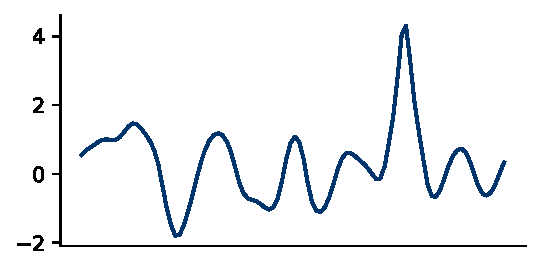
\includegraphics[height=\sampleheight]{figures/task/samples_long/alg5.pdf} &
        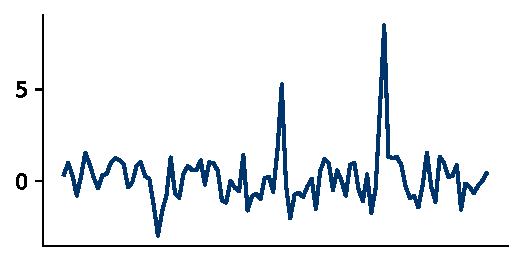
\includegraphics[height=\sampleheight]{figures/task/samples_short/alg5.pdf} &
        \raisebox{38pt}{\rotatebox{90}{\tiny input dimension}} &
        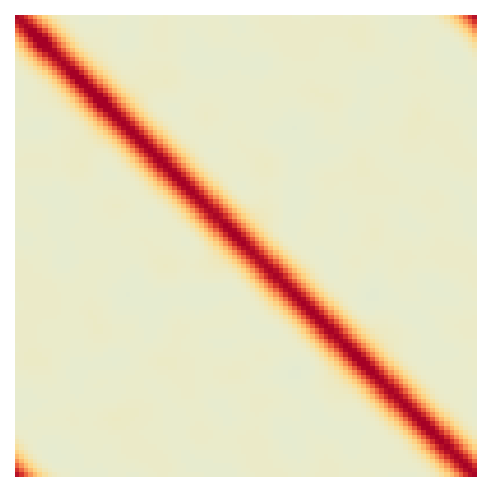
\includegraphics[height=\covheight]{figures/task/cov/alg5.pdf} &
        \raisebox{40pt}{\rotatebox{90}{\tiny $p(X_i)$}} &
        \raisebox{-4pt}{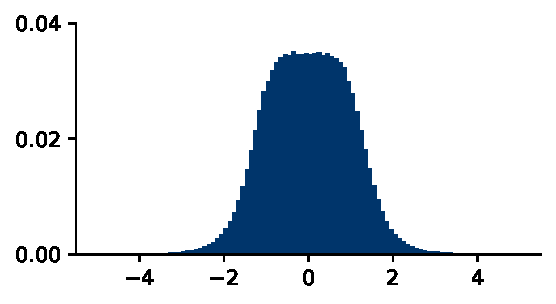
\includegraphics[height=\marginalheight]{figures/task/marginal/alg5.pdf}} \\
        \noalign{\vskip -37pt}
        &&
        \hspace{25pt}\tiny input dimension &
        \hspace{25pt}\tiny input dimension & &
        \hspace{3pt}\tiny input dimension & &
        \hspace{37pt}\tiny input value \\
  \end{tabular}
  \end{centering}
  }
  \caption{
    从左到右:
    长尺度和短尺度样本 $\mathbf{x}$,
    单一尺度的协方差 $\Sigma$,
    以及数据模型的边缘分布 $p(X_i)$,如 \cref{sec:task} 所述:
    Ising 模型(左、右样本分别为 $J=1.2, 0.3$),
    非线性高斯过程~\parencite[NLGP;~][]{ingrosso2022data},
    以及可控峰度模型 \texttt{Kur}
    (左、右样本分别为 $\xi=5, 1$)。
    \emph{
    每个模型生成的样本以零为中心,且其协方差可以被约束为相似,
    但具有不同的高阶统计量,从维度方向的边缘分布中可以看出这一点。
    }
}
  \label{fig:task}
  \vspace{-10pt}
\end{figure}

在 \cref{fig:multi-neuron} 中,我们训练了多个神经元模型,具有 $N=40$ 个输入单元和 $K=10$ 个隐藏单元,所有权重都是可学习的。
一般而言,在第二层中增加灵活性会导致第一层中出现更为多样的结构。
我们在 $\texttt{Kur}(4)$(上)和 $\texttt{Kur}(30)$(下)数据集上进行训练,前者的超峭度为 $3.28$,后者为 $-1.17$。
如同在单神经元模型中一样,前者产生的感受野不具有局部化特征;然而,它们更像是高频振荡而非低频正弦波。
对于 $\texttt{Kur}(30)$,我们预期会出现局部化现象,实际上我们确实看到前三个感受野展现出一定程度的局部化,但其程度低于单神经元模型的表现。
重要的是,并非所有感受野都具有局部化特征,
这是由于第二层权重的变化在实际中改变了引理~\labelcref{lem:varphi} 中三阶导数项中的方差 $\sigma^2$ 所致。

我们进一步将这些预测与 ICA 进行比较,后者是另一种被用于模拟视觉皮层感受野的框架。
我们在 $\texttt{Kur}(3)$ 数据集上进行训练,该数据集的边缘分布具有 $7.66$ 的超峭度,使用 scikit-learn 中的 FastICA 实现拟合了 10 个成分 \parencite{hyvarinen2000independent,scikit-learn}。
我们在 \cref{fig:extensions}(右)中观察到学习到的感受野是局部化的;这与我们的神经网络模型形成对比,后者需要负的超峭度才能实现局部化。
这种差异源于 ICA 的目标是最大化非高斯性,而不关心实现该目标的具体方式。
超峭度的符号在此并不重要,只要它不是零即可。
我们的解析模型与 ICA 之间的这种偏离是一个有趣的未来研究方向,或许可以通过对自然图像的验证来加以探究。
